% !TeX program = lualatex
% !TeX encoding = UTF-8

\documentclass[x11names, border=5pt]{standalone}

\usepackage{fontspec}
\usepackage{unicode-math}
\setmainfont{EB Garamond}
\setsansfont{TeX Gyre Heros}
\setmathfont{Latin Modern Math}

\usepackage{xcolor}
\definecolor{spot}{cmyk}{1,0.20,0,0}
\colorlet{wave}{spot}

\usepackage{tikz}
\usepackage{pgfplots}
\usepgfplotslibrary{polar}

\pgfplotsset{
   compat=1.18,
   wave axis/.style={
      view={0}{90},
      hide axis,
      colormap={diverging}{
         color=(blue!80!black) color=(white) color=(red!80!black)
      },
      point meta min=-1,
      point meta max=1,
      x=1cm, y=1cm, z=0cm,
   },
   wave plot/.style={
      samples=40, samples y=40,
      surf, shader=interp,
      draw=none, % <--- This prevents drawing the black grid lines
   },
}

\begin{document}

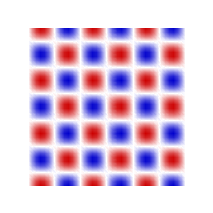
\begin{tikzpicture}
   \begin{axis}[wave axis, width=5cm, height=5cm]
      \addplot3[wave plot, domain=-1:1, domain y=-1:1]
      {sin(deg(3*pi*x))*cos(deg(3*pi*y))};
   \end{axis}
\end{tikzpicture}
\hspace{1cm}
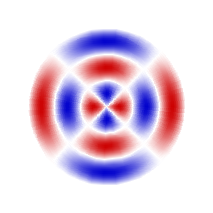
\begin{tikzpicture}
   \begin{axis}[wave axis, width=5cm, height=5cm, data cs=polar]
      \addplot3[wave plot, domain=0:360, domain y=0:1]
      ({x}, {y}, {sin(deg(3*pi*y))*cos(2*x)});
   \end{axis}
\end{tikzpicture}

\end{document}
